\documentclass[oneside]{book}

\setcounter{tocdepth}{1}
\setcounter{secnumdepth}{3}

\usepackage[toc,page]{appendix}
\usepackage{hyperref}
\usepackage[utf8]{inputenc}
\usepackage{graphicx} % Required for the inclusion of images
\usepackage{amsmath} % Required for some math elements 
\usepackage[utf8]{inputenc}
\usepackage[english]{babel}
\newtheorem{theorem}{Theorem}
\newtheorem{corollary}{Corollary}[theorem]
\newtheorem{lemma}[theorem]{Lemma}
\usepackage{listings}
\usepackage{pdfpages}
\usepackage{amssymb}
\usepackage{pdflscape}

\begin{document}

\begin{titlepage}
	\centering
	
\includegraphics[width=0.60\textwidth]{../../logo/UoN_Primary_Logo_RGB.png}\par\vspace{1cm}
	\vspace{1.5cm}
	{\huge\bfseries Comparing Repast Java and Functional Reactive ABS \par}
	\vspace{2cm}
	{\Large\itshape jonathan.thaler@nottingham.ac.uk \par}
	\vfill
	
	\vfill

	{\large \today\par}
\end{titlepage}

\cleardoublepage

\section*{Abstract}
This study we compares the Agent-Based Simulation programming libraries Repast and FrABS. As both are of fundamentally different programming paradigms - Repast uses Java, FrABS Haskell - both propagate fundamental different approaches in implementing ABS. In this document we seek to precicesly identify these fundamental differences, compare them and also look into general benefits and drawbacks of each approach.

\clearpage
\tableofcontents
\clearpage

\section{Introduction}
There exists a large number of simulation packages which allow the convenient creation of System Dynamics simulations by straight-forward visual diagram creation. One simply creates stocks and flows, connects them, specifies the flow-rates and initial parameters and then runs the model. An example for such a visual diagram creation in the simulation package AnyLogic can be seen in Figure \ref{fig:sir_stockflow_diagram}.

\begin{figure}
	\centering
	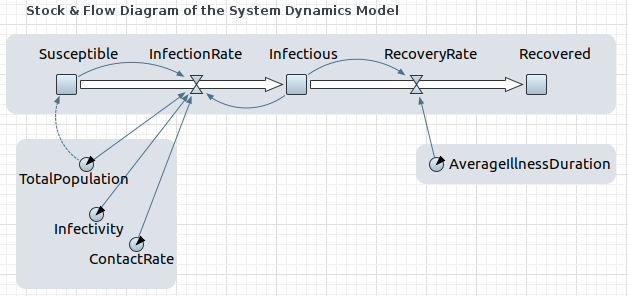
\includegraphics[width=.5\textwidth, angle=0]{./fig/SIR_SD_STOCKFLOW_DIAGRAMM.png}
	\caption{Visual System Dynamics Diagram of the SIR model in AnyLogic Personal Learning Edition 8.3.1.}
	\label{fig:sir_stockflow_diagram}
\end{figure}

Still, implementing System Dynamics directly in code is not as straight forward and involves numerical integration which can be quite tricky to get right. Thus, the aim of this paper is to look into how System Dynamics models can be implemented in code correctly without the use of a simulation package. We use the well known SIR model \cite{kermack_contribution_1927} from epidemiology to demonstrate our approach.

Our language of choice is Haskell because it emphasises a declarative programming style in which one describes \textit{what} instead of \textit{how} to compute. Further it allows to rule out interference with non-deterministic influences or side-effects already at compile-time. This is of fundamental importance for System Dynamics because it behaves completely deterministic and involves no stochastics or non-determinism whatsoever. Also, we make use of Functional Reactive Programming which allows to express continuous-time systems in a functional way. 

We show that by this approach we can arrive at correct-by-construction implementations of System Dynamic models. This means that the correctness of the code is obvious because we have closed the gap between the model specification and its implementation. Thus, the contribution of the paper is the demonstration of how to implement correct-by-construction System Dynamics simulations using Haskell and Functional Reactive Programming.

\chapter{Functional Reactive ABS (FrABS)}
\label{app:frABS}.
In this chapter we present our approach to implementing ABS in the pure functional language Haskell and discuss the issues encountered \footnote{This is not a real paper but only a basic introduction to our approach written for this 1st year report. Thus we assume knowledge of the concept of an agent and ABS already and won't explain these concepts again.}. As already described in our aims and objectives in Chapter \ref{chap:aimsObj}, we are using the functional reactive programming (FRP) paradigm as implemented by the library Yampa and implement an ABS library on top of it \footnote{We have implemented already a prototype together with the Sugarscape-, Agent\_Zero, SIRS- and Schelling-Segregation Model which can be accessed from \url{https://github.com/thalerjonathan/phd/tree/master/coding/libraries/frABS/examples}.}. When comparing our paradigms to the one of object-oriented Java we must solve fundamental problems in rather different ways.

\begin{enumerate}
	\item Representing an agent and environment - there are no classes and objects in Haskell.
	\item Interactions among agents and actions of agents on the environment - there are no method-calls and aliases in Haskell.
	\item Implement the necessary update-strategies as discussed in our paper \ref{app:updateStrategies}, where we only focus on sequential- and parallel-strategies - there is no mutable data which can be changed implicitly through side-effects (e.g. the agents, the list of all the agents, the environment).
\end{enumerate}

Before we can describe how we solved each of the problems, we first need to give an overview of the basic concepts of Yampa.

\section{Yampa}
The central concept of Yampa is the one of a signal-function which can be understood of a mapping from an input-signal to an output-signal. Whether the signal is discrete or continuous does not matter, Yampa is suited equally well to both kinds. Signal-functions are implemented in Yampa using continuations which allow to freeze program-state e.g. through closures and partial applications in functions which can be continued later:
\begin{lstlisting}[]
type DTime = Double

data SF a b = SF { sfTF :: DTime -> a -> (SF a b, b) }
\end{lstlisting}
Such a signal-function, which is called a \textit{transition function} in Yampa, takes the amount of time which has passed since the previous time step and the current input signal (a). It returns a \textit{continuation} of type SF a b determining the behaviour of the signal function on the next step and an output signal (b) of the current time-step. 

Yampa provides a top-level function, running in the IO-Monad, which drives a signal-function by providing both input-values and time-deltas from callbacks. It is important to note that when visualizing a simulation one has in fact two flows of time: the one of the user-interface which always follows real-time flow, and the one of the simulation which could be sped up or slowed down. Thus it is important to note that if I/O of the user-interface (rendering, user-input) occurs within the simulations time-frame then the user-interfaces real-time flow becomes the limiting factor. Yampa provides the function embedSync which allows to embed a signal function within another one which is then run at a given ratio of the outer SF. This allows to give the simulation its own time-flow which is independent of the user-interface. We utilized this in the implementation of Recursive ABS (see Chapter \ref{chap:work}).

Additional functionality which Yampa provides is the concept of Events which allow to implement changing behaviour of signal-functions at given points in time. An event can be understood to be similar to the Maybe-type of Haskell which either is an event with a given type or is simply NoEvent. Yampa provides facilities to detect if an event has fired and also provides functions to switch the signal-function into a new signal-function with changed behaviour. Another feature of Yampa is its EDSL for time-semantics: integration over time, delay, accumulation, holding, firing events after/now/repeatedly.

\section{Agent Representation}
An agent can be seen as a tuple $<id, s, m, ec, b>$.
\begin{itemize}
	\item \textbf{id} - the unique identifier of the agent
	\item \textbf{s} - the generic state of the agent
	\item \textbf{m} - the set of messages the agent understands
	\item \textbf{ec} - the \textit{type} of the environment-cells the agent may act upon
	\item \textbf{b} - the behaviour of the agent
\end{itemize}

\subsection{Id}
The id is simply represented as an Integer and must be unique for all currently existing agents in the system as it is used for message-delivery. A stronger requirement would be that the id of an agent is unique for the whole simulation-run and will never be reused - this would support replications and operations requiring unique agent-ids.

\subsection{State}
Each agent may have a generic state comprised of any data-type, most likely to be a structure.
\begin{lstlisting}[]
data SIRSState = Susceptible | Infected | Recovered
data SIRSAgentState = SIRSAgentState {
    sirsState :: SIRSState,
    sirsCoord :: SIRSCoord,
    sirsTime :: Double
} 
\end{lstlisting}

It is possible that the agent does not rely on any state s, then this will be represented by the unit type (). One wonders if this makes sense and asks how agents can then be distinguished between each other. In functional programming this is easily possible using currying and closures where one encapsulate initial state in the behaviour (see below), which allows to give each agent an individual initial state.

\subsection{Messages}
Agents communicate with each other through messages (see below) and thus need to have an agreed set of messages they understand. This is usually implemented as an ADT.
\begin{lstlisting}[]
data SIRSMsg = Contact SIRSState
\end{lstlisting}

\subsection{Environment-Cell}
The agent needs to know the generic type of the cells the environment is made of to be able to act upon the environment. Note that at the moment we only implemented a discrete 2d environment and provide only access and manipulation to the cells in a 2D discrete fashion. In the case of a continuous n-dimensional environment this approach needs to be thoroughly revised. It is important to understand that it is the \textit{type} of the cells and not the environment itself.

\subsection{Behaviour}
The behaviour of the agent is a signal-function which maps an AgentIn-Signal to an AgentOut-Signal. It has the following signature: 
\begin{lstlisting}[]
type AgentBehaviour s m e = SF (AgentIn s m e) (AgentOut s m e)
\end{lstlisting}

AgentIn provides the necessary data to the agent-behaviour: its id, incoming messages, the current state s, the environment (made out of the cells ec), its position in the environment and a random-number generator. 

AgentOut allows the agent to communicate changes out of the behaviour: kill itself, create new agents, sending messages, state s, environment (made out of the cells ec), environment-position and random-number generator. 

\section{Environment}
So far we only implemented a 2d-discrete environment. It can be understood to be a tuple of $<b, l, n, w, cs>$.
\begin{itemize}
	\item \textbf{b} - the optional behaviour of the environment
	\item \textbf{l} - the limit of the environment: its maximum boundary extending from (0,0)
	\item \textbf{n} - the neighbourhood of the environment (e.g. Neumann, Moore, Manhattan...)
	\item \textbf{w} - the wrapping-type of the environment (clipping, horizontal, vertical, both)
	\item \textbf{cs} - the cells of the environment of type c
\end{itemize}

We represent the environment-behaviour as a signal-function as well but one which maps an environment to itself. It has the following signature:
\begin{lstlisting}[]
type EnvironmentBehaviour c = SF (Environment c) (Environment c)
\end{lstlisting}
This is a regular SF thus having also the time of the simulation available and is called after all agents are updated. Note that the environment cannot send messages to agents because it is not an agent itself. An example of an environment behaviour would be to regrow some good on each cell according to some rate per time-unit (inspired by SugarScape regrowing of Sugar).

The cells are represented as a 2-dimensional array with indices from (0,0) to limit and a cell of type c at every position. Note that the cell-type c is the same environment-cell type ec of the agent.

Each agent has a copy of the environment passed in through the AgentIn and can change it by passing a changed version of the environment out through AgentOut.

\section{Messaging}
As discussed in the literature reflection in Chapter \ref{chap:refl}, inspired by the actor model we will resort to synchronized, reliable message passing with share nothing semantics to implement agent-agent interactions. Each Agent can send a message to an other agent through AgentOut-Signal where the messages are queued in the AgentIn-Signal and can be processed when the agent is updated the next time. The agent is free to ignore the messages and if it does not process them they will be simply lost.
Note that due to the fact we don't have method-calls in FP, messaging will always take some time, which depends on the sampling interval of the system. This was not obviously clear when implementing ABS in an object-oriented way because there we can communicate through method calls which are a way of interaction which takes no simulation-time.

%TODO: Push vs. Pull. we need push because we need to 'sample' the system at regular time-intervals because agent-behaviour can depend on time as well (pro-active) and not only on messaging. if we had only the latter, a pull approach would suffice.

% my wrongthinking: messaging ALWAYS takes time e.g. send/response roundtrip. conversations dont take time but are restricted for the receiver e.g. the receiver cannot send messages to others or change the environment in a conversation

% because an agent cannot reply within the same timestep sampling interval becomes an issue: if we need a reply within a given time then the sampling interval needs to be at least twice as much
% difference between discrete and continuous: the successor of discrete is defined whereas in the case of continuous it is not? how is the successor defined in the case of continuous time?

\section{Conversations}
The messaging as implemented above works well for one-directional, virtual asynchronous interaction where we don't need a reply at the same time. A perfect use-case for messaging is making contact with neighbours in the SIRS-model: the agent sends the contact message but does not need any response from the receiver, the receiver handles the message and may get infected but does not need to communicate this back to the sender. 
A different case is when agents need to transact in the time-step one or multiple times: agent A interacts with agent B where the semantics of the model (and thus messaging) need an immediate response from agent B - which can lead to further interactions initiated by agent A. The Sugarscape model has three use-cases for this: sex, warfare and trading amongst agents all need an immediate response (e.g. wanna mate with me?, I just killed you, wanna trade for this price?). The reason is that we need to transact now as all of the actions only work on a 1:1 relationship and could violate resource-constraints.
For this we introduce the concept of a conversation between agents. This allows an agent A to initiate a conversation with another agent B in which the simulation is virtually halted and both can exchange an arbitrary number of messages through calling and responding without time passing (something not possible without this concept because in each iteration the time advances). After either one agent has finished with the conversation it will terminate it and the simulation will continue with the updated agents (note the importance here: \textit{both} agents can change their state in a conversation). The conversation-concept is implemented at the moment in the way that the initiating agent A has all the freedom in sending messages, starting a new conversation,... but that the receiving agent B is only able to change its state but is not allowed to send messages or start conversations in this process. Technically speaking: agent A can manipulate an AgentOut whereas agent B can only manipulate its next AgentIn.
When looking at conversations they may look like an emulation of method-calls but they are more powerful: a receiver can be unavailable to conversations or simply refuse to handle this conversation. This follows the concept of an active actor which can decide what happens with the incoming interaction-request, instead of the passive object which cannot decide whether the method-call is really executed or not.

\section{Iteration-Strategies}
Building on the foundations laid out in my paper about iteration-strategies in Appendix \ref{app:updateStrategies}, we implement two of the four strategies: sequential- and parallel-strategy. We deliberately ignore the concurrent- and actor-strategy for now and leave this for further research \footnote{Also both strategies would require running in the STM-Monad, which is not possible with Yampa. The work of Ivan Perez in \cite{perez_functional_2016} implemented a library called Dunai, which is the same as Yampa but capable of running in an arbitrary Monad.}.
Implementing iteration-strategies using Haskell and FRP is not as straight-forward as in e.g. Java because one does not have mutable data which can be updated in-place. Although my work on programming paradigms in Appendix \ref{app:paradigms} did not take FRP into account, general concepts apply equally as well.

\subsection{Sequential}
In this strategy the agents are updated one after another where the changes (messages sent, environment changed,...) of one agent are visible to agents updated after. Basically this strategy is implemented as a variant of fold which allows to feed output of one agent (e.g. messages and the environment) forward to the other agents while iterating over the list of agents. For each agent the agent-behaviour signal-function is called with the current AgentIn as input to retrieve the according AgentOut. The messages of the AgentOut are then distributed to the receivers AgentIn.
The environment of the agent, which is passed in through AgentIn and returned through AgentOut will then be passed forward to all agents i + 1 AgentIn in the current iteration and override their old environment. Thus all steps of changes made to the environment are visible in the AgentOuts. The last environment is then the final environment in the current iteration and will be returned by the callback function together with the current AgentOuts.

\subsection{Parallel}
The parallel strategy is \textit{much} easier to implement than the sequential but is of course not applicable to all models because of it different semantics. Basically this strategy is implemented as a map over all agents which calls each agent-behaviour signal-function with the agents AgentIn to retrieve the new AgentOut. Then the messages are distributed amongst all agents.
A problem in this strategy is that the environment is duplicated to each agent and then each agent can work on it and return a changed environment. Thus after one iteration there are n versions of environments where n is equals to the number of agents. These environments must then be collapsed into a final one which is always domain-specific thus needs to be done through a function provided in the environment itself.

%TODO: functionsl approach to ABS: parallel application to previous states where only one agent is acting and the others are fixed. per step we have n results. for a full iteration we need $(n-1)^2$ applicatioms

\section{Further Research}
In his 1st year report about Functional Reactive GUI programming, Ivan Perez \footnote{main author of the paper \cite{perez_functional_2016}} writes: "FRP tries to shift the direction of data-flow, from message passing onto data dependency. This helps reason about what things are over time, as opposed to how changes propagate". This of course raises the question whether FRP is \textit{really} the right approach, because the way we implement ABS, message-passing is an essential concept. It is important to emphasis that agent-relations in interactions are never fixed in advance and are completely dynamic, forming a network. Maybe one has to look at message passing in a different way in FRP, and to view and model it as a data-dependency but it is not clear how this can be done. The question is whether there is a mechanism in which we have explicit data-dependency but which is dynamic like message-passing but does not try to fake method-calls? Maybe the concept of conversations (see above) are a way to go but we leave this for further research at the moment.

\chapter{Repast Java}

\section{JZombies}

\subsection{Repast Java}

\subsection{FrABS}
Parallel vs. Sequential
	-> Sequential is as in Repast
	-> Parallel is novel, but need to collapse environment: but how?

needed to implement standard-cells in discrete2d:
	-> empty / non-empty with single / multiple occupier
	-> supply helper-functions
		-> occupy / unoccupy / isoccupied
		-> allOccupiers
	-> supply functions which construct these discrete2d with standard-cells

agents are implemented as the union of ADT

\subsection{Comparing dynamics}
Both use the same parameters, the one specified in the Repast Example.

FrABS leads much faster to a full infection: in case of using shuffling we arrive at full infection around 80 steps. When NOT using shuffling, is is happening around 140 steps.

Repast Java leads to a full infection after around 200 steps.

I think the reason for this is a different scheduling for the human agents. The zombies agents move in every time step but the humans have a watch added which gets triggered as soon as a zombie enters their moore-neighbourhood:
$
		@Watch(watcheeClassName = "jzombies.Zombie", 
			watcheeFieldNames = "moved",
			query = "within_moore 1", 
			whenToTrigger = WatcherTriggerSchedule.IMMEDIATE)$
Thus humans are scheduled right after an approaching zombie which allows them to flee thus prolonging the time until all humans are infected thus impacting the dynamics. In the case of FrABS the result is that although this specific zombie who enters the moore-neighbourhood does not directly pose a threat for the human as this human is still on another patch, until the human is scheduled, other zombies can close in thus reducing the action-radius of the human considerably.

This Watcher-Mechanism is not possible in FrABS and there are no plans to implement such as it would need a completely different approach. Also we cannot think of a mechnism which allows to specify such a meta-programming construct in Haskell.

\section{SIR System Dynamics}

\subsection{Repast Java}
\url{https://repast.github.io/docs/RepastSystemDynamicsGettingStarted.pdf}

\subsection{FrABS}

\section{SIR Agent-Based Simulation}

\subsection{Repast Java}

\subsection{FrABS}

\section{Case Study II: Sugarscape}
\label{sec:sugarscape_concurrent}
The second case study is the Sugarscape model as introduced in Chapter \ref{sec:sugarscape}. In this case study we look into the potential performance improvement in a model with much more complex agent behaviour and dramatically increased writes on the shared environment.

We implemented the \textit{Carrying Capacity} (p. 30) section of Chapter II of the Sugarscape book \cite{epstein_growing_1996}. In each step agents search (move) to the cell with the most sugar they see within their vision, harvest all of it from the environment and consume sugar because of their metabolism. Sugar regrows in the environment over time. Only one agent can occupy a cell at a time. Agents don't age and cannot die from age. If agents run out of sugar due to their metabolism, they die from starvation and are removed from the simulation. The authors report that the initial number of agents quickly drops and stabilises around a level depending on the model parameters. This is in accordance with our results as we show in Chapter \ref{ch:property} and guarantees that we don't run out of agents. The model parameters are as follows:

\begin{itemize}
	\item Sugar Endowment: each agent has an initial sugar endowment randomly uniform distributed between 5 and 25 units;
	\item Sugar Metabolism: each agent has a sugar metabolism randomly uniform distributed between 1 and 5;
	\item Agent Vision: each agent has a vision randomly uniform distributed between 1 and 6, same for each of the 4 directions (N, W, S, E);
	\item Sugar Growback: sugar grows back by 1.0 unit per step until the maximum capacity of a cell is reached;
	\item Agent Number: initially 500 agents;
	\item Environment Size: 50 x 50 cells with toroid boundaries which wrap around in both x and y dimension.
\end{itemize}

Note that in this implementation (as in the full Chapter II of the book), no direct and no synchronous agent-interactions as we implemented them in Chapter \ref{sec:eventdriven_implementation} are happening. As in the SIR example, all agents interact with each other indirectly through the shared environment. This allows us to regard the implementation as a time-driven, parallel one wherein each step agents act conceptually at the same time.

We compare four different implementations \footnote{The code is freely available at \url{https://github.com/thalerjonathan/phd/tree/master/public/stmabs/code/SugarScape}}:

\begin{enumerate}
	\item Sequential - All agents are run after another (including the environment) and the environment is shared amongst the agents using a \textit{StateT} transformer.
	\item Lock-Based - All agents are run concurrently in the \textit{IO} monad and the environment is shared between the agents, using an \textit{IORef} with the access synchronised through an \textit{MVar} lock.
	\item STM TVar - All agents are run concurrently in the \textit{STM} monad and the environment is shared using a \textit{TVar} between the agents.
	\item STM TArray - All agents are run concurrently in the \textit{STM} monad and the environment is shared using a \textit{TArray} between the agents. 
\end{enumerate}

We follow \cite{lysenko_framework_2008} and measure the average number of steps per second of the simulation over 60 seconds. For each experiment we conducted 8 runs on our machine (see Table \ref{tab:machine_specs}) under no additional work-load and report the average. In the experiments we varied the number of cores when running concurrently - the numbers are always indicated clearly.

%\paragraph{Output} Note that we omit the graphical rendering in the functional approach because it is a serious bottleneck taking up substantial amount of the simulation time. Although visual output is often important in ABS, it is not what we are interested here thus we completely omit it and only output the number of agents in the simulation at each step piped into a file, thus omitting slow output to the console \footnote{Note that we need to produce \textit{some} output because of Haskells laziness - if we wouldn't output anything from the simulation then the expressions would actually never be fully evaluated thus resulting in high number of steps per second but which obviously don't really reflect the true computations done.}.

\paragraph{Ordering} The model specification requires to shuffle agents before every step (Footnote 12 on page 26 \cite{epstein_growing_1996}). In the \textit{Sequential} approach we do this explicitly but in the \textit{Lock-Based} and both \textit{STM} approaches we assume this to happen automatically due to race-conditions in concurrency, thus we arrive at an effectively shuffled processing of agents: we implicitly assume that the order of the agents is \textit{effectively} random in every step. The important difference between the two approaches is that in the \textit{Sequential} approach we have full control over this randomness but in the \textit{STM} not - also this means that repeated runs with the same initial conditions might lead to slightly different results. 
This decision leaves the execution order of the agents ultimately to Haskell's Runtime System and the underlying OS. We are aware that by doing this, we make assumptions that the threads run uniformly distributed (fair) but such assumptions should not be made in concurrent programming. As a result we can expect this fact to produces non-uniform distributions of agent runs but we assumed that for this model this does not has a significance influence - in case of doubt, we could resort to shuffling the agents before running them in every step. We agree that this very problem would deserve in-depth research on its own, where also the influence of non-deterministic ordering on the correctness and results of ABS has to be analysed. This is not the main interest of this section though and we leave it for further research as it is completely beyond the focus of this thesis.

%Note that in the concurrent implementations we have two options for running the environment: either asynchronously as a concurrent agent at the same time with the population agents or synchronously after all agents have run. We must be careful though as running the environment as a concurrent agent can be seen as conceptually wrong because the time when the regrowth of the sugar happens is now completely random. In this case it could happen that sugar regrows in the very first transaction or in the very last, different in each step, which can be seen as a violation of the model specifications. Thus we do not run the environment concurrently with the agents but synchronously after all agents have run.

\subsection{Constant Agent Size}
In a first approach we compare the performance of all implementations on varying numbers of cores. The results are reported in Table \ref{tab:varying_cores} and plotted in Figure \ref{fig:varying_cores}. 

\begin{table}
	\centering
	\begin{tabular}{cc|c|c}
		\multicolumn{1}{ c||  }{\multirow{2}{*}{} } &
		\multicolumn{1}{ |c| }{Cores} & Steps & Retries      \\ \hline \hline 
		
		\multicolumn{1}{ c||  }{\multirow{1}{*}{Sequential} } &
		\multicolumn{1}{ |c| }{1} & 39.4 & N/A     \\ \hline \hline 
		
		\multicolumn{1}{ c||  }{\multirow{4}{*}{Lock-Based} } &
		\multicolumn{1}{ |c| }{1} & 43.0 & N/A       \\ \cline{2-4}
		\multicolumn{1}{ c||  }{}                       &
		\multicolumn{1}{ |c| }{2} & 51.8 & N/A   \\ \cline{2-4}
		\multicolumn{1}{ c||  }{}                       &
		\multicolumn{1}{ |c| }{3} & 57.4 & N/A   \\ \cline{2-4}
		\multicolumn{1}{ c||  }{}                       &
		\multicolumn{1}{ |c| }{4} & 58.1 & N/A   \\ \hline \hline 
		
		\multicolumn{1}{ c||  }{\multirow{4}{*}{STM \textit{TVar}} } &
		\multicolumn{1}{ |c| }{1} & \textbf{47.3} & 0.0       \\ \cline{2-4}
		\multicolumn{1}{ c||  }{}                       &
		\multicolumn{1}{ |c| }{2} & 53.5 & 1.1    \\ \cline{2-4}
		\multicolumn{1}{ c||  }{}                       &
		\multicolumn{1}{ |c| }{3} & 57.1 & 2.2    \\ \cline{2-4}
		\multicolumn{1}{ c||  }{}                       &
		\multicolumn{1}{ |c| }{4} & 53.0 & 3.2   \\ \hline \hline 
		
		\multicolumn{1}{ c||  }{\multirow{4}{*}{STM \textit{TArray}} } &
		\multicolumn{1}{ |c| }{1} & 45.4 & 0.0       \\ \cline{2-4}
		\multicolumn{1}{ c||  }{}                       &
		\multicolumn{1}{ |c| }{2} & \textbf{65.3} & 0.02   \\ \cline{2-4}
		\multicolumn{1}{ c||  }{}                       &
		\multicolumn{1}{ |c| }{3} & \textbf{75.7} & 0.04    \\ \cline{2-4}
		\multicolumn{1}{ c||  }{}                       &
		\multicolumn{1}{ |c| }{4} & \textbf{84.4} & 0.05   \\ \hline \hline 
	\end{tabular}  	
  	
  	\caption{Steps per second and retries on 50x50 grid with 500 initial agents on varying cores.}
	\label{tab:varying_cores}
\end{table}

\begin{figure}
	\centering
	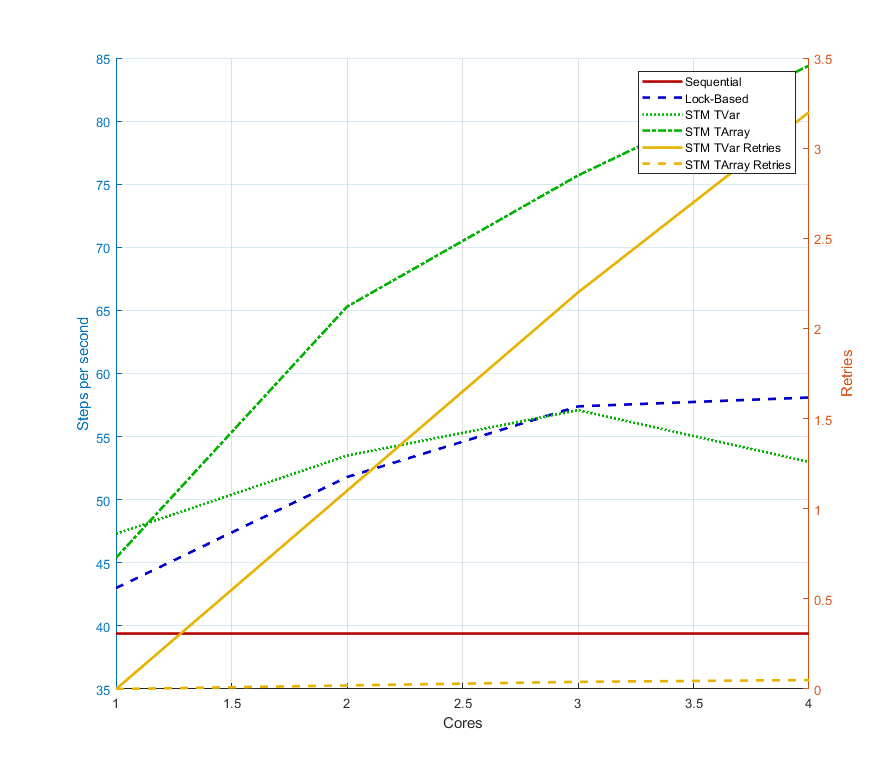
\includegraphics[width=0.7\textwidth, angle=0]{./fig/concurrentabs/sugarscape/varying_cores.png}
	\caption{Steps per second and retries on 50x50 grid and 500 initial agents on varying cores.}
	\label{fig:varying_cores}
\end{figure}

As expected, the \textit{Sequential} implementation is the slowest, followed by the \textit{Lock-Based} and \textit{TVar} approach whereas \textit{TArray} is the best performing one.

We clearly see that using a \textit{TVar} to share the environment is a very inefficient choice in this model: \textit{every} write to a cell leads to a retry independent whether the reading agent reads that changed cell or not, because the data-structure can not distinguish between individual cells. By using a \textit{TArray} we can avoid the situation where a write to a cell in a far distant location of the environment will lead to a retry of an agent which never even touched that cell. Also the \textit{TArray} seems to scale up by 10 steps per second for every core added. It will be interesting to see how far this could go with the Amazon experiment, as we seem not to hit a limit with 4 cores yet.

The inefficiency of \textit{TVar} is also reflected in the nearly similar performance of the \textit{Lock-Based} implementation which even outperforms it on 4 cores. This is due to very similar approaches because both operate on the whole environment instead of only the cells as \textit{TArray} does. This seems to be a bottleneck in \textit{TVar} reaching the best performance on 3 cores, which then drops on 4 cores due to an increasing retries ratio. The \textit{Lock-Based} approach seems to reduce its returns on increased number of cores hitting a limit at 4 cores as well.

\subsection{Scaling up Agents}
So far we kept the initial number of agents at 500, which due to the model specification, quickly drops and stabilises around 200 due to the carrying capacity of the environment as described in the book \cite{epstein_growing_1996} section \textit{Carrying Capacity} (p. 30).

We now want to measure the performance of our approaches under increased number of agents. For this we slightly change the implementation: always when an agent dies it spawns a new one which is inspired by the ageing and birthing feature of Chapter III in the book \cite{epstein_growing_1996}. This ensures that we keep the number of agents roughly constant (still fluctuates but doesn't drop to low levels) over the whole duration. This ensures a constant load of concurrent agents interacting with each other and demonstrates also the ability to terminate and create concurrent agents (threads) dynamically during the simulation.

Except for the \textit{Sequential} approach we ran all experiments with 4 cores (TVar with 3 as well). We looked into the performance of 500, 1,000, 1,500, 2,000 and 2,500 (maximum possible capacity of the 50x50 environment). The results are reported in Table \ref{tab:state_results_agentsscale_time} and plotted in Figure \ref{fig:state_results_agentsscale_time}.

\begin{table}
	\centering
  	\begin{tabular}{ c || c | c | c | c | c }
        Agents  & Sequential & Lock-Based & TVar (3 cores) & TVar (4 cores) & TArray  \\ \hline \hline 
    	    500     & 14.4       & 20.2		  &	20.1           & 18.5       	& \textbf{71.9}    \\ \hline
   		1,000   & 6.8        & 10.8 	      & 10.4           & 9.5         & \textbf{54.8}    \\ \hline
   		1,500   & 4.7        & 8.1 		  & 7.9            & 7.3			& \textbf{44.1}    \\ \hline
   		2,000   & 4.4        & 7.6 		  & 7.4            & 6.7    		& \textbf{37.0}    \\ \hline 
   		2,500   & 5.3        & 5.4 		  & 9.2            & 8.9			& \textbf{33.3}    \\ \hline \hline
   	\end{tabular}
  	
  	\caption{Steps per second on 50x50 grid with varying number of agents with 4 (and 3) cores except Sequential (1 core).}
	\label{tab:state_results_agentsscale_time}
\end{table}

\begin{figure}
	\centering
	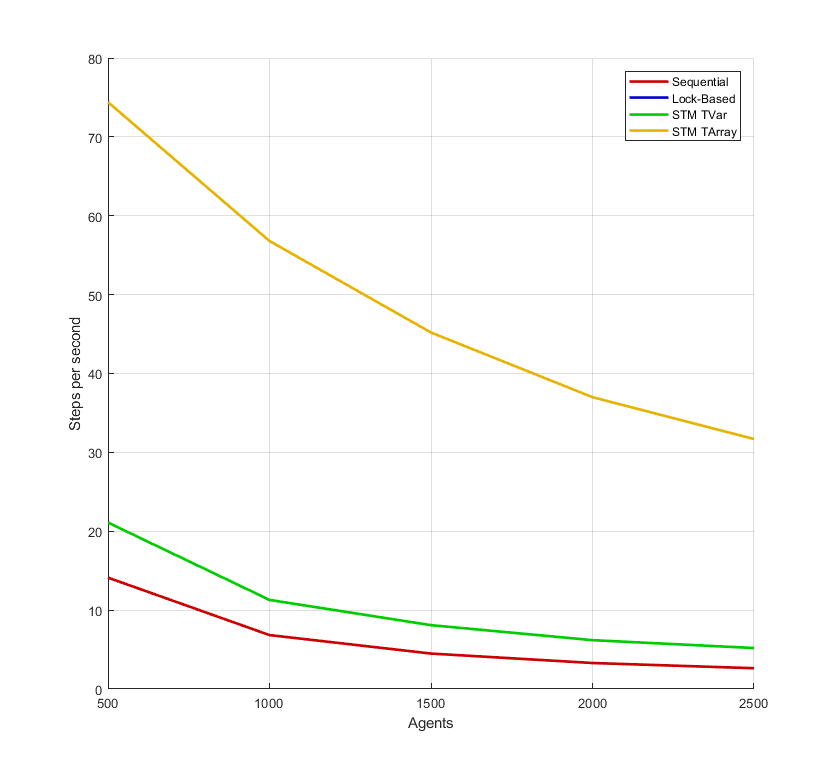
\includegraphics[width=1.0\textwidth, angle=0]{./fig/concurrentabs/sugarscape/varying_agents.png}
	\caption{Steps per second on 50x50 grid and varying number of agents with 4 (and 3) cores except Sequential (1 core).}
	\label{fig:state_results_agentsscale_time}
\end{figure}

As expected, the \textit{TArray} implementation outperforms all others substantially. Also as expected, the \textit{TVar} implementation on 3 cores is faster than on 4 cores as well when scaling up to more agents. The \textit{Lock-Based} approach performs about the same as the \textit{TVar} on 3 cores because of the very similar approaches: both access the \textit{whole} environment. Still the \textit{TVar} approach uses one core less to arrive at the same performance, thus strictly speaking outperforming the \textit{Lock-Based} implementation.

What seems to be very surprising is that in the \textit{Sequential} and \textit{TVar} cases the performance with 2,500 agents is \textit{better} than the one with 2,000 agents. The reason for this is that in the case of 2,500 agents, an agent can't move anywhere because all cells are already occupied. In this case the agent won't rank the cells in order of their pay-off (max sugar) to move to but just stays where it is. We hypothesize that due to Haskells laziness the agents actually never look at the content of the cells in this case but only the number which means that the cells themselves are never evaluated which further increases performance. This leads to the better performance in case of \textit{Sequential} and \textit{TVar} because both exploit laziness.
In the case of the \textit{Lock-Based} approach we still arrive at a lower performance because the limiting factor are the unconditional locks. In the case of the \textit{TArray} approach we also arrive at a lower performance because it seems that STM perform reads on the neighbouring cells which are not subject to lazy evaluation. In Haskell it is notoriously difficult to reason about efficiency (see Chapter \ref{ch:drawbacks} for a short discussion on drawbacks) and this behaviour of improved performance due to Haskells lazyness is no exception. We leave an in-depth investigation for further research as it is beyond the focus of this chapter.

We also measured the average retries both for \textit{TVar} and \textit{TArray} under 2,500 agents where the \textit{TArray} approach shows best scaling performance with 0.01 retries whereas \textit{TVar} averages at 3.28 retries. Again this can be attributed to the better transactional data-structure which reduces retry-ratio substantially to near-zero levels.

\subsection{Going Large-Scale}
To test how far we can scale up the number of cores in both the \textit{Lock-Based} and \textit{TArray} cases, we ran the two experiments (carrying capacity and rebirthing) on Amazon EC2 instances with increasing number of cores starting with 16 and 32 to see if we run into decreasing returns. The results are reported in Table \ref{tab:sug_varying_cores_amazon}.

\begin{table}
	\centering
%  	\begin{tabular}{ c || c | c | c }
%                   & Cores & Carrying Capacity & Rebirthing  \\ \hline \hline 
%    	Lock-Based & 16    & 53.9              & 4.4         \\ \hline
%    	Lock-Based & 32    & 44.2              & 3.6         \\ \hline \hline 
%   		
%   		STM TArray & 16    & \textbf{116.8} (0.23)      & \textbf{39.5} (0.08) \\ \hline
%   		STM TArray & 32    & 109.8 (0.41)      & 31.3 (0.18) \\ \hline \hline 
%   	\end{tabular}
  	
	\begin{tabular}{cc|c|c}
		\multicolumn{1}{ c||  }{\multirow{2}{*}{} } &
		\multicolumn{1}{ |c| }{Cores} & Carrying Capacity    & Rebirthing       \\ \hline \hline 
		
		\multicolumn{1}{ c||  }{\multirow{2}{*}{Lock-Based} } &
		\multicolumn{1}{ |c| }{16} & 53.9              & 4.4       \\ \cline{2-4}
		\multicolumn{1}{ c||  }{}                       &
		\multicolumn{1}{ |c| }{32} & 44.2              & 3.6      \\ \hline \hline 
		
		\multicolumn{1}{ c||  }{\multirow{2}{*}{STM TArray} } &
		\multicolumn{1}{ |c| }{16} & \textbf{116.8} (0.23)      & \textbf{39.5} (0.08)       \\ \cline{2-4}
		\multicolumn{1}{ c||  }{}                       &
		\multicolumn{1}{ |c| }{32} & \textbf{109.8} (0.41)      & \textbf{31.3} (0.18)      \\ \hline \hline 
	\end{tabular}  	
  	
  	\caption{Steps per second on varying cores on Amazon S2 Services.}
	\label{tab:sug_varying_cores_amazon}
\end{table}

As expected, the \textit{Lock-Based} approach doesn't scale up to many cores because each additional core brings more contention to the lock, resulting in even more decreased performance. This is particularly obvious in the rebirthing experiment because of the much larger number of concurrent agents. The \textit{TArray} approach returns better performance on 16 cores but fails to scale further up to 32 where the performance drops below the one with 16 cores. We indicated the retry-ratio in brackets and see that they roughly double from 16 to 32, which is the reason why performance drops as at this point. 

%the INCREASE in time can only happen due to more retries
%Carrying Capacity 16 core ~ 0.23 retry-ratio
%Carrying Capacity 32 core ~ 0.41 retry-ratio
%
%Rebirthing 16 core ~ 0.08 retry-ratio
%Rebirthing 32 core ~ 0.18 retry-ratio

\subsection{Comparison with other approaches}
The paper \cite{lysenko_framework_2008} reports a performance of 17 steps in RePast, 18 steps in MASON (both non-parallel) and 2,000 steps per second on a GPU on a 128x128 grid. Although our \textit{Sequential} implementation, which runs non-parallel as well, outperforms the RePast and MASON implementations of \cite{lysenko_framework_2008}, one must be very well aware that these results were generated in 2008, on current hardware of that time.

%When we run the SugarScape example of RePast with the same model parameters as ours on the same machine (see Table \ref{tab:machine_specs}) we arrive at roughly 450 steps per second - a factor of about 3.8 faster than even our STM \textit{TArray} implementation on 16 cores. This might seem quite shocking, even more so because RePast also performs visual output, rendering the SugarScape in every step. When scaling up the agents to 2,500 the RePast version arrives around roughly 95 steps per second which is still faster by a factor of 3 than our 4 core \textit{TArray} implementation. We attribute this substantial performance difference to the inherent performance difference of functional programming to imperative approaches as already outlined in the previous section. 

The very high performance on the GPU does not concern us here as it follows a very different approach than ours. We focus on speeding up implementations on the CPU as directly as possible without locking overhead. When following a GPU approach one needs to map the model to the GPU which is a delicate and non-trivial matter. With our approach we show that speed up with concurrency is very possible without the low-level locking details or the need to map to GPU. Also some features as bilateral trading between agents, where a pair of agents needs to come to a conclusion over multiple synchronous steps, is difficult to implement on a GPU whereas this is easily possible using STM.

Note that we kept the grid-size constant because we implemented the environment as a single agent which works sequentially on the cells to regrow the sugar. Obviously this doesn't really scale up on parallel hardware and experiments which we haven't included here due to lack of space, show that the performance goes down dramatically when we increase the environment to 128x128 with same number of agents which is the result of Amdahl's law where the environment becomes the limiting factor of the simulation. Depending on the underlying data-structure used for the environment we have two options to solve this problem. In the case of the \textit{Sequential} and \textit{TVar} implementation we build on an indexed array, which we can be updated in parallel using the existing data-parallel support in Haskell. In the case of the \textit{TArray} approach we have no option but to run the update of every cell within its own thread. We leave both for further research as it is out of scope of this paper.

\subsection{Discussion}
This case study showed clearly that besides being substantially faster than the \textit{Sequential} implementation, \textit{STM} is also able to perform considerably better than a \textit{Lock-Based} approach even in the case of a model with much higher complexity in agent behaviour and dramatically increased number of writes to the environment.
Further, this case study demonstrated that the selection of the right transactional data-structure is of fundamental importance when using \textit{STM}. Selecting the right transactional data-structure is very model-specific and can lead to dramatically different performance results.
In this case the \textit{TArray} performed best due to many writes but in the SIR case-study a \textit{TVar} showed good enough results due to the very low number of writes. When not carefully selecting the right transactional data-structure which supports fine-grained concurrency, a lock-based implementation might perform as well or even outperform the STM approach as can be seen when using the \textit{TVar}.
Although the \textit{TArray} is the better transactional data-structure overall, it might come with an overhead, performing worse on low number of cores than a \textit{TVar} approach but has the benefit of quickly scaling up to multiple cores. Depending on the transactional data-structure, scaling up to multiple cores hits a limit at some point. In the case of the \textit{TVar} the best performance is reached with 3 cores. With the \textit{TArray} we reached this limit around 16 cores.

Note that the comparison between the \textit{Lock-Based} approach and the \textit{STM TArray} implementation is a bit unfair due to a very different locking structure. A more suitable comparison would have been to use an indexed Array with a tuple of (MVar, IORef) in each cell to support fine-grained locking on cell-level. This would be a more just comparison to the \textit{STM Array} where fine-grained transactions happen on the cell-level. We hypothesize that \textit{STM} will still outperform the \textit{IO} approach but to a lesser degree - we leave the proof of this for further research.

%Unfortunately, for this model the performance is nowhere comparable to imperative approaches, which we attribute to the inherent performance difference of functional programming to imperative approaches. With the use of advanced language features we might arrive at much improved performance but we leave this for further research as we focus primarily on the comparison between lock-based and STM approaches.

%we can implement everything except synchronous direct agent-interactions atm: if agent-interaction is one-way e.g. paying back a loan then this is no problem. thus the following parts of the Sugarscape are not possible with our current STM approach: mating, trading and lending  because all 3 require direct agent-to-agent interaction over multiple steps. We leave the problem of developing such an algorithm / implementation for further research.

\renewcommand\bibname{References}

\bibliographystyle{acm}
\bibliography{../../references/phdReferences}

\end{document}
